\documentclass{article}
\usepackage[utf8]{inputenc} %кодировка
\usepackage[T2A]{fontenc}
\usepackage[english,russian]{babel} %русификатор 
\usepackage{mathtools} %библиотека матеши
\usepackage[left=1cm,right=1cm,top=2cm,bottom=2cm,bindingoffset=0cm]{geometry} %изменение отступов на листе
\usepackage{amsmath}
\usepackage{graphicx} %библиотека для графики и картинок
\graphicspath{}
\DeclareGraphicsExtensions{.pdf,.png,.jpg}
\usepackage{subcaption}
\usepackage{pgfplots}
\usepackage{float}

\begin{document}
% НАЧАЛО ТИТУЛЬНОГО ЛИСТА
\begin{center}
    \Large
    Федеральное государственное автономное \\
    образовательное учреждение высшего образования \\ 
    «Научно-образовательная корпорация ИТМО»\\
    \vspace{0.5cm}
    \large
    Факультет программной инженерии и компьютерной техники \\
    Направление подготовки 09.03.04 Программная инженерия \\
    \vspace{1cm}
    \Large
    \textbf{Отчёт по лабораторной работе №2} \\
        По дисциплине «Компьютерные сети» ( семестр 6)\\
    \large
    \vspace{8cm}

    \begin{minipage}{.33\textwidth}
    \end{minipage}
    \hfill
    \begin{minipage}{.4\textwidth}
    
        \textbf{Студент}: \vspace{.1cm} \\
        \ Дениченко Александр P3312\\
        \textbf{Практик}:  \\
        \ Тропченко Андрей Александрович
    \end{minipage}
    \vfill
Санкт-Петербург\\ 2025 г.
\end{center}
\pagestyle{empty}
% КОНЕЦ ТИТУЛЬНОГО ЛИСТА 
\newpage
\pagestyle{plain}

\section*{Цель работы}
Изучение принципов настройки и функционирования локальных сетей,
построенных с использованием концентраторов и коммутаторов, а также
процессов передачи данных на основе стека протоколов TCP/IP, с
использованием программы моделирования компьютерных сетей NetEmul.
\begin{itemize}
    \item построить три модели локальной сети: с использованием концентратора,
    коммутатора и многосегментную сеть;
    \item выполнить настройку сети, заключающуюся в присвоении IP-адресов
    интерфейсам сети;
    \item выполнить тестирование разработанных сетей путем проведения
    экспериментов по передаче данных (пакетов и кадров) на основе
    протоколов UDP и TCP;
    \item проанализировать результаты тестирования и сформулировать выводы об
    эффективности смоделированных вариантов построения локальных сетей;
    \item сохранить разработанные модели локальных сетей для демонстрации
    процессов передачи данных при защите лабораторной работы.
\end{itemize}

\section*{Вариант}

Ф=9; И=9; О=8; Н=12
\\ 
сети 1 = 2
\\
сети 2 = 4
\\
сети 3 = 3
\\
Класс IP-адресов = В
\\
для класса В:
(И+Н+128).(О+Н).(Ф+Н).(Ф+И) = (9+12+128).(8+12).(9+12).(9+9) = 149.20.21.18 (диапазон от 128 до 191)

\section{Построение сети с концентратором}

Для построения сети пронумеруем интерфейсы компьютеров: 149.20.21.18 и 149.20.21.19



\end{document}
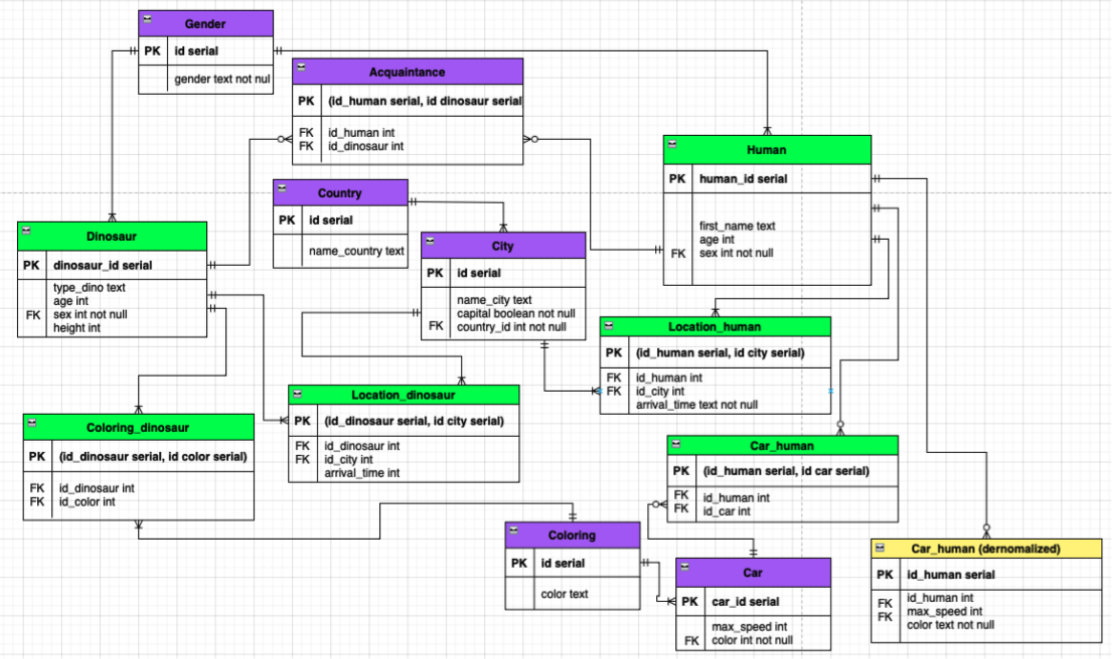
\includegraphics[width=.9\textwidth]{123}